%%%%%%%%%%%%%%%%%%%%%%%%%%%%%%%%%%%%
% Lesson Plan (50 minutes)
%%%%%%%%%%%%%%%%%%%%%%%%%%%%%%%%%%%%
\begin{frame}
    \frametitle{Lesson Plan}
    \begin{itemize}
        \item xx min Lecture: review from last time
        \begin{itemize}
            \item We should (now) be very comfortable with Z- and t-tests, and we recently learned how to compare 2 means
            \item Recall that ANOVA allows us to compare 3+ means in different levels/categories, for example in <lecture example>
            \item Review F-statistic
        \end{itemize}
        \item xx min Lecture: p-value meaning in this case (like slide 71)
        \item xx min Edfinity quiz: now with all the tools in hand, conduct an ANOVA test for the lecture example, step-by-step
        \item xx min R Demonstration: answers to the quiz in R, and review interpretation of the test results
    \end{itemize}
\end{frame}

%%%%%%%%%%%%%%%%%%%%%%%%%%%%%%%%%%%%
% Learning objectives:
%%%%%%%%%%%%%%%%%%%%%%%%%%%%%%%%%%%%
\begin{frame}
    \frametitle{Learning Objectives}
    \begin{itemize}
        \item \textbf{M1, LO3: Use R for Data Management and Exploration:} Utilize R to load, pre-process, and explore data through visualization and summarization techniques.
        \item \textbf{M3, LO1: Understand Point Estimates and Sampling Variability:} Define a sample statistic (point estimate) for a population parameter, and explain how it varies across different samples.
        \item \textbf{M3, LO3: Calculate and Interpret Standard Error:} Calculate the standard error for proportions and interpret it as a measure of sampling variability.
        \item \textbf{M3, LO4: Explain Hypothesis Testing and Its Limitations:} Discuss the use cases and potential issues with hypothesis testing, including the interpretation of results.
        \item \textbf{M3, LO6: Distinguish Statistical vs. Practical Significance:} Differentiate between statistical significance and practical significance, and explain the implications of each.
        \item \textbf{M4, LO2: Design and Interpret Confidence Intervals:} Design, execute, and interpret confidence intervals for the population proportion.
        \item \textbf{M4: LO8: Conduct and Interpret ANOVA:} Assess whether conditions for an ANOVA are met, and if so, design, execute, and interpret the test to compare sample means across several groups.
    \end{itemize}
\end{frame}
    
%%%%%%%%%%%%%%%%%%%%%%%%%%%%%%%%%%%%
% TODO: Copy and adapt these slides base on the lesson plan
%%%%%%%%%%%%%%%%%%%%%%%%%%%%%%%%%%

\section{Comparing means with ANOVA}

%%%%%%%%%%%%%%%%%%%%%%%%%%%%%%%%%%%

\subsection{Aldrin in the Wolf River}

%%%%%%%%%%%%%%%%%%%%%%%%%%%%%%%%%%%

\begin{frame}
\frametitle{}

\begin{center}
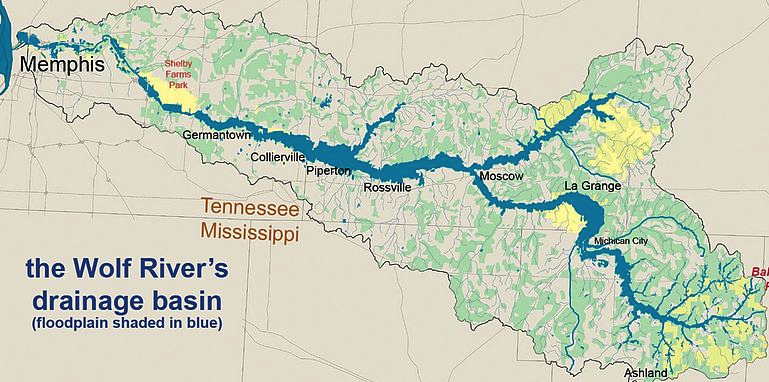
\includegraphics[width=0.5\textwidth]{7-5_anova/figures/aldrin/wolf}
\end{center}

{\small
\begin{itemize}

\item  The Wolf River in Tennessee flows past an abandoned site once used by the pesticide industry for dumping wastes, including chlordane (pesticide), aldrin, and dieldrin (both insecticides).

\pause

\item These highly toxic organic compounds can cause various cancers and birth defects.

\pause

\item The standard methods to test whether these substances are present in a river is to take samples at six-tenths depth. 

\pause

\item But since these compounds are denser than water and their molecules tend to stick to particles of sediment, they are more likely to be found in higher concentrations near the bottom than near mid-depth.

\end{itemize}
}

\end{frame}

%%%%%%%%%%%%%%%%%%%%%%%%%%%%%%%%%%%

\begin{frame}
\frametitle{Data}

Aldrin concentration (nanograms per liter) at three levels of depth. \\

\begin{center}
\begin{tabular}{r | c | c}
\hline
 	& aldrin 					& depth \\ 
\hline
1 	& \textcolor{darkGray}{3.80} 	& \textcolor{darkGray}{bottom}  \\ 
2 	& \textcolor{darkGray}{4.80} 	& \textcolor{darkGray}{bottom}  \\ 
...	&						& \\
10	& \textcolor{darkGray}{8.80} 	& \textcolor{darkGray}{bottom} \\
11	& \textcolor{blue}{3.20} 		& \textcolor{blue}{middepth}  \\
12	& \textcolor{blue}{3.80} 		& \textcolor{blue}{middepth} \\
...	&						& \\
20 	& \textcolor{blue}{6.60} 		& \textcolor{blue}{middepth} \\
21	& \textcolor{oiB}{3.10} 		& \textcolor{oiB}{surface} \\
22	& \textcolor{oiB}{3.60} 		& \textcolor{oiB}{surface} \\
...	&						& \\
30 	& \textcolor{oiB}{5.20} 		& \textcolor{oiB}{surface} \\  
\hline
\end{tabular}
\end{center}

\end{frame}

%%%%%%%%%%%%%%%%%%%%%%%%%%%%%%%%%%%

\begin{frame}
\frametitle{Exploratory analysis}

Aldrin concentration (nanograms per liter) at three levels of depth. \\

\begin{center}
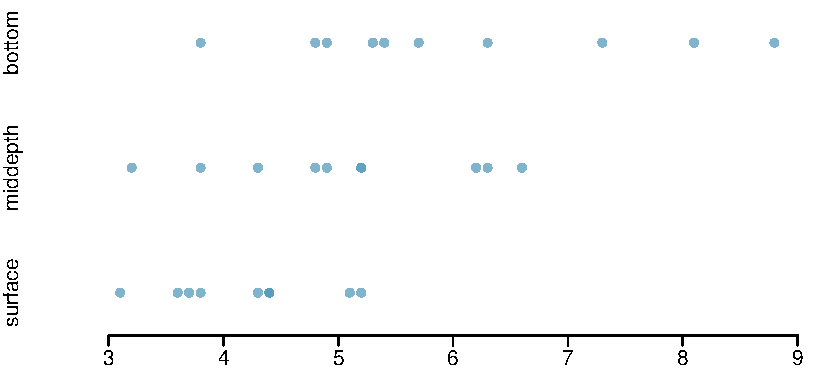
\includegraphics[width=0.75\textwidth]{7-5_anova/figures/aldrin/dotplot}
\end{center}

\begin{center}
\begin{tabular}{l | c c c}
		& n	& mean	& sd		\\
\hline
bottom	& 10	& 6.04	& 1.58 \\
middepth& 10	& 5.05	& 1.10 \\
surface	& 10	& 4.20	& 0.66 \\
\hline
overall	& 30	& 5.1	0	& 1.37
\end{tabular}
\end{center}

\end{frame}

%%%%%%%%%%%%%%%%%%%%%%%%%%%%%%%%%%%

\begin{frame}
\frametitle{Research question}

\dq{Is there a difference between the mean aldrin concentrations among the three levels?}

\vspace{0.5cm}

\pause

\begin{itemize}

\item To compare means of 2 groups we use a Z or a T statistic.

\pause

\item To compare means of 3+ groups we use a new test called \hl{ANOVA} and a new statistic called \hl{F}.

\end{itemize}

\end{frame}

%%%%%%%%%%%%%%%%%%%%%%%%%%%%%%%%%%%

\begin{frame}
\frametitle{ANOVA}

ANOVA is used to assess whether the mean of the outcome variable is different for different levels of a categorical variable.

\pause

\begin{itemize}
\item[] \mathhl{H_0:} The mean outcome is the same across all categories, 
\[\mu_1 = \mu_2 = \cdots = \mu_k, \]
where $\mu_i$ represents the mean of the outcome for observations in category $i$.
\item[]
\item[] \mathhl{H_A:} At least one mean is different than others.
\end{itemize}

\end{frame}

%%%%%%%%%%%%%%%%%%%%%%%%%%%%%%%%%%%

\begin{frame}
\frametitle{Conditions}

\begin{enumerate}

\item The observations should be independent within and between groups

\begin{itemize}
\item If the data are a simple random sample from less than 10\% of the population, this condition is satisfied.
\item Carefully consider whether the data may be independent (e.g. no pairing). 
\item Always important, but sometimes difficult to check.
\end{itemize}

\pause

\item The observations within each group should be nearly normal.

\begin{itemize}
\item Especially important when the sample sizes are small.
\end{itemize}

\dq{How do we check for normality?}

\pause

\item The variability across the groups should be about equal.

\begin{itemize}
\item Especially important when the sample sizes differ between groups.
\end{itemize}

\dq{How can we check this condition?}

\end{enumerate}

\end{frame}

%%%%%%%%%%%%%%%%%%%%%%%%%%%%%%%%%%%

\begin{frame}
\frametitle{$z$/$t$ test vs. ANOVA - Purpose}

\twocol{0.5}{0.5}
{
\[ \hl{$z$/$t$ test} \]
Compare means from \hl{two} groups to see whether they are so far apart that the observed difference cannot reasonably be attributed to sampling variability.
\[ H_0: \mu_1 = \mu_2 \]
}
{
\[ \hl{ANOVA} \]
Compare the means from \hl{two or more} groups to see whether they are so far apart that the observed differences cannot all reasonably be attributed to sampling variability.
\[ H_0: \mu_1 = \mu_2 = \cdots = \mu_k \]
}

\end{frame}

%%%%%%%%%%%%%%%%%%%%%%%%%%%%%%%%%%%

\begin{frame}
\frametitle{$z$/$t$ test vs. ANOVA - Method}

\twocol{0.5}{0.5}
{
\[ \hl{$z$/$t$ test} \]
Compute a test statistic (a ratio).
\[ z / t = \frac{(\bar{x}_1 - \bar{x}_2) - (\mu_1 - \mu_2)}{SE(\bar{x}_1 - \bar{x}_2)} \]
}
{
\[ \hl{ANOVA} \]
Compute a test statistic (a ratio).
\[ F = \frac{\text{variability bet. groups}}{\text{variability w/in groups}} \]
}

\vspace{1cm}

\pause

\begin{itemize}

\item Large test statistics lead to small p-values. 

\item If the p-value is small enough $H_0$ is rejected, we conclude that the population means are not equal.

\end{itemize}

\end{frame}

%%%%%%%%%%%%%%%%%%%%%%%%%%%%%%%%%%%

\begin{frame}
\frametitle{$z$/$t$ test vs. ANOVA}

\begin{itemize}

\item With only two groups t-test and ANOVA are equivalent, but only if we use a pooled standard variance in the denominator of the test statistic.

\pause

\item With more than two groups, ANOVA compares the sample means to an overall \hl{grand mean}.

\end{itemize}

\end{frame}

%%%%%%%%%%%%%%%%%%%%%%%%%%%%%%%%%%%

\begin{frame}
\frametitle{Hypotheses}

\pq{What are the correct hypotheses for testing for a difference between the mean aldrin concentrations among the three levels?}

\begin{enumerate}[(a)]
\item $H_0: \mu_B = \mu_M = \mu_S$ \\
$H_A: \mu_B \ne \mu_M \ne \mu_S$ \\
\item $H_0: \mu_B \ne \mu_ M \ne \mu_S$ \\
$H_A: \mu_B = \mu_M = \mu_S$ \\
\solnMult{$H_0: \mu_B = \mu_M = \mu_S$ \\
$H_A:$ At least one mean is different.}
\item $H_0: \mu_B = \mu_M = \mu_S = 0$ \\
$H_A:$ At least one mean is different.
\item $H_0: \mu_B = \mu_M = \mu_S$ \\
$H_A: \mu_B > \mu_M > \mu_S$ \\
\end{enumerate}

\end{frame}

%%%%%%%%%%%%%%%%%%%%%%%%%%%%%%%%%%%

\subsection{ANOVA and the F test}

%%%%%%%%%%%%%%%%%%%%%%%%%%%%%%%%%%%

\begin{frame}
\frametitle{Test statistic}

\dq{Does there appear to be a lot of variability within groups? How about between groups?}

\[ F = \frac{\text{variability bet. groups}}{\text{variability w/in groups}}  \]

\begin{center}
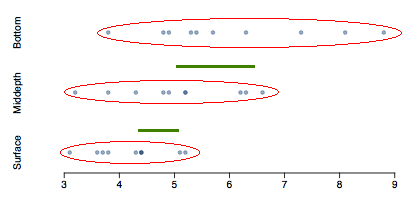
\includegraphics[width=0.75\textwidth]{7-5_anova/figures/aldrin/dotplot_var}
\end{center}

\end{frame}

%%%%%%%%%%%%%%%%%%%%%%%%%%%%%%%%%%%

%\begin{frame}
%\frametitle{Test statistic (cont.)}
%
%\[ F = \frac{\text{variability bet. groups}}{\text{variability w/in groups}} = \frac{\hl{MSG}}{\hl{MSE}}  \]
%
%\begin{itemize}
%
%\item \hl{MSG} is mean square between groups
%\[ df_G = k - 1 \]
%where $k$ is number of groups
%
%\item \hl{MSE} is mean square error - variability in residuals
%\[ df_E = n - k \]
%where $n$ is number of observations.
%
%\end{itemize}
%
%\end{frame}
%
%%%%%%%%%%%%%%%%%%%%%%%%%%%%%%%%%%%%

\begin{frame}
\frametitle{$F$ distribution and p-value}

\[ F =  \frac{\text{variability bet. groups}}{\text{variability w/in groups}} \]

\vspace{-1cm}

\begin{center}
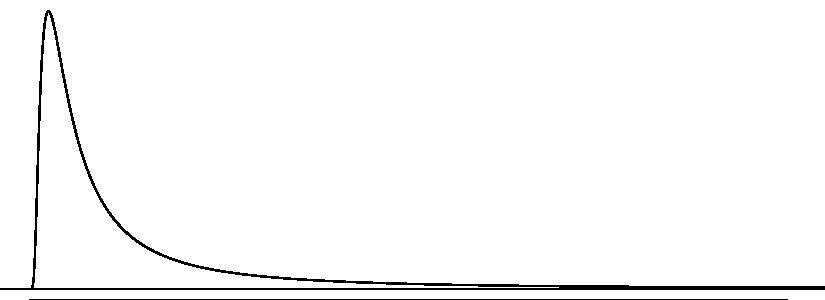
\includegraphics[width=0.75\textwidth]{7-5_anova/figures/fdist/fdist}
\end{center}

\begin{itemize}

\item In order to be able to reject $H_0$, we need a small p-value, which requires a large F statistic.

\item In order to obtain a large F statistic, variability between sample means needs to be greater than variability within sample means.

\end{itemize}

\end{frame}

%%%%%%%%%%%%%%%%%%%%%%%%%%%%%%%%%%%

\subsection{ANOVA output, deconstructed}

%%%%%%%%%%%%%%%%%%%%%%%%%%%%%%%%%%%

\begin{frame}
\frametitle{}

\vspace{-0.5cm}

{\footnotesize
\begin{center}
\begin{tabular}{ll >{\columncolor[gray]{.6}[.5\tabcolsep]}rrrrr}
\hline
 			& 			& Df 	& Sum Sq	& Mean Sq 	& F value 	& Pr($>$F) \\ 
\hline
(\hl{G}roup) 	& depth 		& 2 	& 16.96 	& 8.48 		& 6.13 	& 0.0063 \\ 
(\hl{E}rror) 	& Residuals 	& 27 	& 37.33 	& 1.38 		&  		&  \\ 
\hline
	 		& \hl{T}otal	& 29	& 54.29 \\
\end{tabular}
\end{center}
}

\formula{Degrees of freedom associated with ANOVA}
{
\begin{itemize}
\item groups: $df_G = k - 1$, where $k$ is the number of groups
\item total: $df_T = n - 1$, where $n$ is the total sample size
\item error: $df_E = df_T - df_G$
\end{itemize}
}

\pause

\begin{itemize}

\item $df_G = k - 1 = 3 - 1 = 2$ \\ 

\pause

\item $df_T = n - 1 = 30 - 1 = 29$

\pause

\item $df_E = 29 - 2 = 27$ \\

\end{itemize}

\end{frame}

%%%%%%%%%%%%%%%%%%%%%%%%%%%%%%%%%%%

\begin{frame}
\frametitle{}

\vspace{-0.25cm}

{\footnotesize
\begin{center}
\begin{tabular}{ll r>{\columncolor[gray]{.6}[.5\tabcolsep]}rrrr}
\hline
 			& 			& Df 	& Sum Sq	& Mean Sq 	& F value 	& Pr($>$F) \\ 
\hline
(\hl{G}roup) 	& depth 		& 2 	& \orange{16.96} 	& 8.48 		& 6.13 	& 0.0063 \\ 
(\hl{E}rror) 	& Residuals 	& 27 	& 37.33 	& 1.38 		&  		&  \\ 
\hline
	 		& \hl{T}otal	& 29	& 54.29 \\
\end{tabular}
\end{center}
}

\formula{Sum of squares between groups, SSG}
{
Measures the variability between groups 
\vspace{-0.25cm}
\[ SSG = \sum_{i = 1}^{k} n_i (\bar{x}_i - \bar{x})^2 \]
where $n_i$ is each group size, $\bar{x}_i$ is the average for each group, $\bar{x}$ is the overall (grand) mean.
}

\pause

\vspace{-0.5cm}

\twocol{0.4}{0.5}
{
{\small
\begin{center}
\begin{tabular}{l | c c }
		& n	& mean		\\
\hline
bottom	& 10	& 6.04	 \\
middepth& 10	& 5.05	 \\
surface	& 10	& 4.2	 \\
\hline
overall	& 30	& 5.1	
\end{tabular}
\end{center}
}
}
{
\pause
\begin{eqnarray*}
SSG &=& \pr{ 10 \times (6.04 - 5.1)^2 } \\
\pause
&+& \pr{ 10 \times (5.05 - 5.1)^2 } \\
\pause
&+& \pr{ 10 \times (4.2 - 5.1)^2 } \\
\pause
&=& 16.96 \\
\end{eqnarray*}
}

\end{frame}

%%%%%%%%%%%%%%%%%%%%%%%%%%%%%%%%%%%

\begin{frame}
\frametitle{}

\vspace{-0.25cm}

{\footnotesize
\begin{center}
\begin{tabular}{ll r>{\columncolor[gray]{.6}[.5\tabcolsep]}rrrr}
\hline
 			& 			& Df 	& Sum Sq	& Mean Sq 	& F value 	& Pr($>$F) \\ 
\hline
(\hl{G}roup) 	& depth 		& 2 	& 16.96	& 8.48 		& 6.13 	& 0.0063 \\ 
(\hl{E}rror) 	& Residuals 	& 27 	& 37.33 	& 1.38 		&  		&  \\ 
\hline
	 		& \hl{T}otal	& 29	& \orange{54.29} \\
\end{tabular}
\end{center}
}

\formula{Sum of squares total, SST}
{
Measures the variability between groups 
\vspace{-0.25cm}
\[ SST = \sum_{i = 1}^{n} (x_i - \bar{x}) \]
where $x_i$ represent each observation in the dataset.
}

\pause

\vspace{-0.75cm}

\begin{eqnarray*}
SST &=& (3.8 - 5.1)^2 + (4.8 - 5.1)^2 + (4.9 - 5.1)^2 + \cdots + (5.2 - 5.1)^2 \\
\pause
&=& (-1.3)^2 + (-0.3)^2 + (-0.2)^2 + \cdots + (0.1)^2 \\
\pause
&=& 1.69 + 0.09 + 0.04 + \cdots + 0.01 \\
\pause
&=& 54.29
\end{eqnarray*}

\end{frame}

%%%%%%%%%%%%%%%%%%%%%%%%%%%%%%%%%%%

\begin{frame}
\frametitle{}

\vspace{-0.25cm}

{\footnotesize
\begin{center}
\begin{tabular}{ll r>{\columncolor[gray]{.6}[.5\tabcolsep]}rrrr}
\hline
 			& 			& Df 	& Sum Sq	& Mean Sq 	& F value 	& Pr($>$F) \\ 
\hline
(\hl{G}roup) 	& depth 		& 2 	& 16.96	& 8.48 		& 6.13 	& 0.0063 \\ 
(\hl{E}rror) 	& Residuals 	& 27 	& \orange{37.33} 	& 1.38 		&  		&  \\ 
\hline
	 		& \hl{T}otal	& 29	& 54.29 \\
\end{tabular}
\end{center}
}

\formula{Sum of squares error, SSE}
{
Measures the variability within groups:
\[ SSE = SST - SSG \]
}

\pause

\[ SSE =  54.29 - 16.96 =  37.33 \]

\end{frame}

%%%%%%%%%%%%%%%%%%%%%%%%%%%%%%%%%%%

\begin{frame}
\frametitle{}

\vspace{-0.25cm}

{\footnotesize
\begin{center}
\begin{tabular}{ll rr>{\columncolor[gray]{.6}[.5\tabcolsep]}rrr}
\hline
 			& 			& Df 	& Sum Sq	& Mean Sq 	& F value 	& Pr($>$F) \\ 
\hline
(\hl{G}roup) 	& depth 		& 2 	& 16.96	& \orange{8.48} 		& 6.13 	& 0.0063 \\ 
(\hl{E}rror) 	& Residuals 	& 27 	& 37.33 	& \orange{1.38} 		&  		&  \\ 
\hline
	 		& \hl{T}otal	& 29	& 54.29 \\
\end{tabular}
\end{center}
}

\formula{Mean square error}
{
Mean square error is calculated as sum of squares divided by the degrees of freedom.
}

\pause

\begin{eqnarray*}
MSG &=& 16.96 / 2 = 8.48 \\
\pause
MSE &=& 37.33 / 27 = 1.38
\end{eqnarray*}

\end{frame}

%%%%%%%%%%%%%%%%%%%%%%%%%%%%%%%%%%%

\begin{frame}
\frametitle{}

\vspace{-0.25cm}

{\footnotesize
\begin{center}
\begin{tabular}{ll rrr>{\columncolor[gray]{.6}[.5\tabcolsep]}rr}
\hline
 			& 			& Df 	& Sum Sq	& Mean Sq 	& F value 	& Pr($>$F) \\ 
\hline
(\hl{G}roup) 	& depth 		& 2 	& 16.96	& 8.48 		& \orange{6.14} 	& 0.0063 \\ 
(\hl{E}rror) 	& Residuals 	& 27 	& 37.33 	& 1.38 		&  		&  \\ 
\hline
	 		& \hl{T}otal	& 29	& 54.29 \\
\end{tabular}
\end{center}
}

\formula{Test statistic, F value}
{
As we discussed before, the F statistic is the ratio of the between group and within group variability.
\[ F = \frac{MSG}{MSE} \]
}

\pause

\[ F = \frac{8.48}{1.38} = 6.14 \]

\end{frame}

%%%%%%%%%%%%%%%%%%%%%%%%%%%%%%%%%%%

\begin{frame}
\frametitle{}

\vspace{-0.25cm}

{\footnotesize
\begin{center}
\begin{tabular}{ll rrr>{\columncolor[gray]{.6}[.5\tabcolsep]}rr}
\hline
 			& 			& Df 	& Sum Sq	& Mean Sq 	& F value 	& Pr($>$F) \\ 
\hline
(\hl{G}roup) 	& depth 		& 2 	& 16.96	& 8.48 		& \orange{6.14} 	& 0.0063 \\ 
(\hl{E}rror) 	& Residuals 	& 27 	& 37.33 	& 1.38 		&  		&  \\ 
\hline
	 		& \hl{T}otal	& 29	& 54.29 \\
\end{tabular}
\end{center}
}

\formula{p-value}
{
p-value is the probability of at least as large a ratio between the ``between group" and ``within group" variability, if in fact the means of all groups are equal. It's calculated as the area under the F curve, with degrees of freedom $df_G$ and $df_E$, above the observed F statistic.
}

\pause

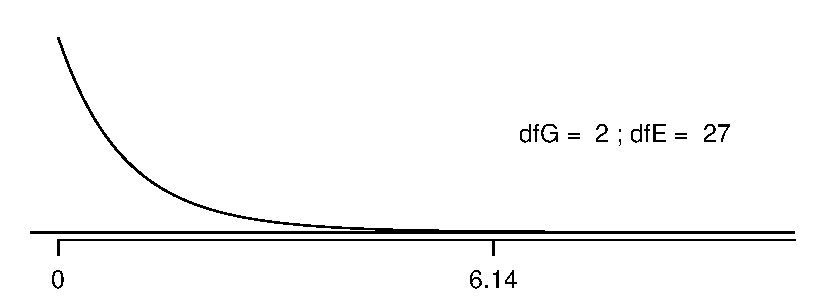
\includegraphics[width=0.9\textwidth]{7-5_anova/figures/aldrin/f}

\end{frame}

%%%%%%%%%%%%%%%%%%%%%%%%%%%%%%%%%%%

\begin{frame}
\frametitle{Conclusion - in context}

\pq{What is the conclusion of the hypothesis test?}

$\:$ \\

The data provide convincing evidence that the average aldrin concentration
\begin{enumerate}[(a)]

\item  is different for all groups.

\item on the surface is lower than the other levels.

\solnMult{is different for at least one group.}

\item is the same for all groups.

\end{enumerate}

\end{frame}

%%%%%%%%%%%%%%%%%%%%%%%%%%%%%%%%%%%

\begin{frame}
\frametitle{Conclusion}

\begin{itemize}

\item  If p-value is small (less than $\alpha$), reject $H_0$. The data provide convincing evidence that at least one mean is different from (but we can't tell which one).

\pause

\item If p-value is large, fail to reject $H_0$. The data do not provide convincing evidence that at least one pair of means are different from each other, the observed differences in sample means are attributable to sampling variability (or chance).

\end{itemize}

\end{frame}

%%%%%%%%%%%%%%%%%%%%%%%%%%%%%%%%%%%

\subsection{Checking conditions}

%%%%%%%%%%%%%%%%%%%%%%%%%%%%%%%%%%%

\begin{frame}[fragile]
\frametitle{(1) independence}

\dq{Does this condition appear to be satisfied?}

\soln{\only<2>{In this study the we have no reason to believe that the aldrin concentration won't be independent of each other.}}

\end{frame}

%%%%%%%%%%%%%%%%%%%%%%%%%%%%%%%%%%%

\begin{frame}[fragile]
\frametitle{(2) approximately normal}

\dq{Does this condition appear to be satisfied?}

\begin{center}
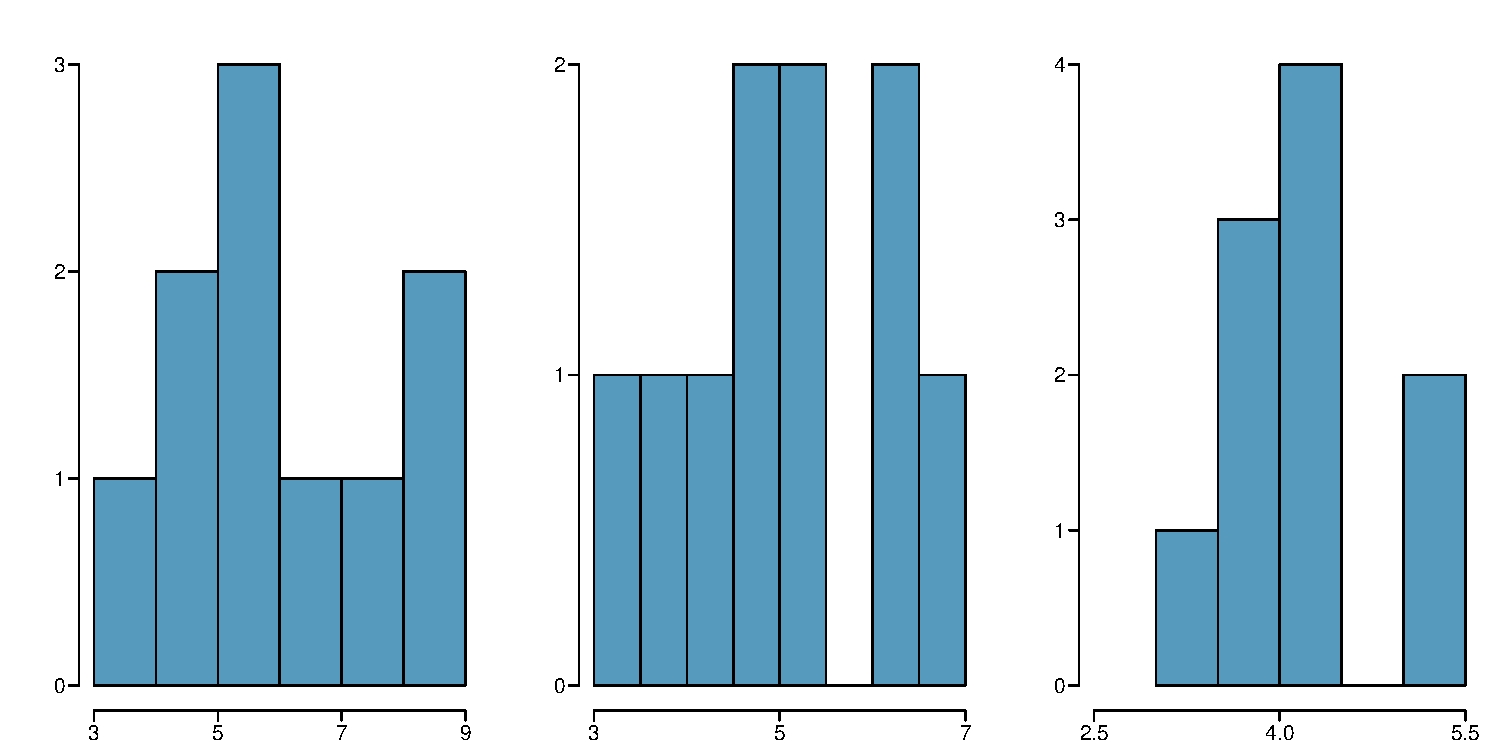
\includegraphics[width=\textwidth]{7-5_anova/figures/aldrin/normal}
\end{center}

\end{frame}

%%%%%%%%%%%%%%%%%%%%%%%%%%%%%%%%%%%

\begin{frame}[fragile]
\frametitle{(3) constant variance}

\dq{Does this condition appear to be satisfied?}

\begin{center}
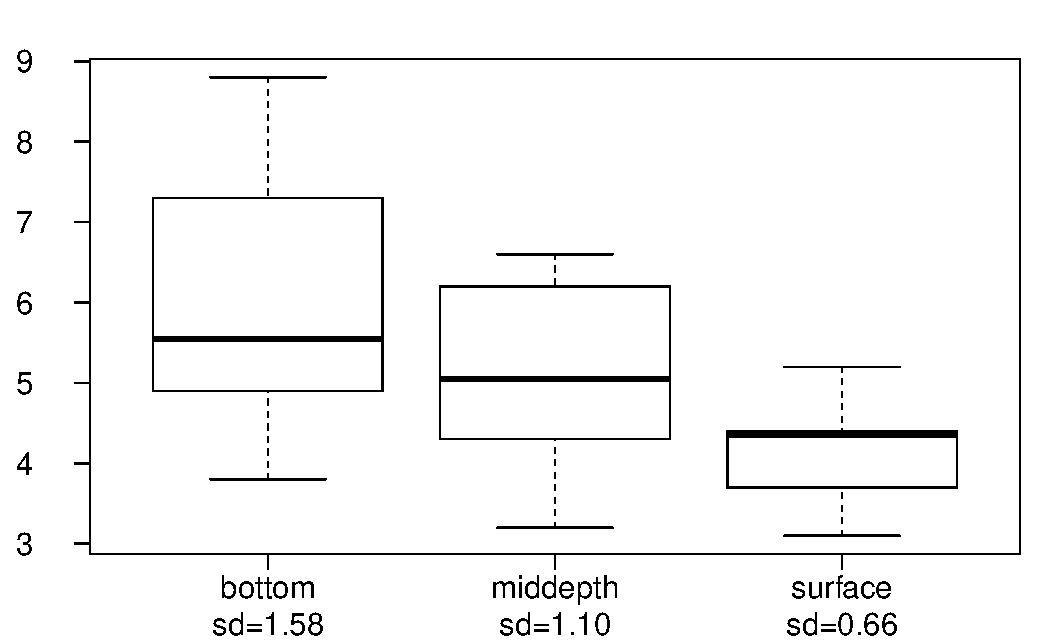
\includegraphics[width=0.7\textwidth]{7-5_anova/figures/aldrin/homo}
\end{center}

\end{frame}

%%%%%%%%%%%%%%%%%%%%%%%%%%%%%%%%%%%

\subsection{Multiple comparisons \& Type 1 error rate}

%%%%%%%%%%%%%%%%%%%%%%%%%%%%%%%%%%%

\begin{frame}
\frametitle{Which means differ?}

\begin{itemize}

\item Earlier we concluded that at least one pair of means differ. The natural question that follows is ``which ones?"

\pause

\item We can do two sample $t$ tests for differences in each possible pair of groups.

\pause

\end{itemize}

\dq{Can you see any pitfalls with this approach?}

\pause

\begin{itemize}

\item When we run too many tests, the Type 1 Error rate increases.

\item This issue is resolved by using a modified significance level.

\end{itemize}

\end{frame}

%%%%%%%%%%%%%%%%%%%%%%%%%%%%%%%%%%%

\begin{frame}
\frametitle{Multiple comparisons}

\begin{itemize}

\item The scenario of testing many pairs of groups is called \hl{multiple comparisons}.

\pause

\item The \hl{Bonferroni correction} suggests that a more \orange{stringent} significance level is more appropriate for these tests:

\[ \alpha^\star = \alpha / K \]

where $K$ is the number of comparisons being considered.

\pause

\item If there are $k$ groups, then usually all possible pairs are compared and $K = \frac{k (k - 1)}{2}$.

\end{itemize}

\end{frame}

%%%%%%%%%%%%%%%%%%%%%%%%%%%%%%%%%%%

\begin{frame}
\frametitle{Determining the modified $\alpha$}

\pq{In the aldrin data set depth has 3 levels: bottom, mid-depth, and surface. If $\alpha = 0.05$, what should be the modified significance level for two sample $t$ tests for determining which pairs of groups have significantly different means?}

\begin{enumerate}[(a)]
\item $\alpha^* = 0.05$
\item $\alpha^* = 0.05 / 2 = 0.025$
\solnMult{$\alpha^* = 0.05 / 3 = 0.0167$}
\item $\alpha^* = 0.05 / 6 = 0.0083$
\end{enumerate}

\end{frame}

%%%%%%%%%%%%%%%%%%%%%%%%%%%%%%%%%%%

\begin{frame}
\frametitle{Which means differ?}

\pq{Based on the box plots below, which means would you expect to be significantly different?}

\twocol{0.6}{0.4}{
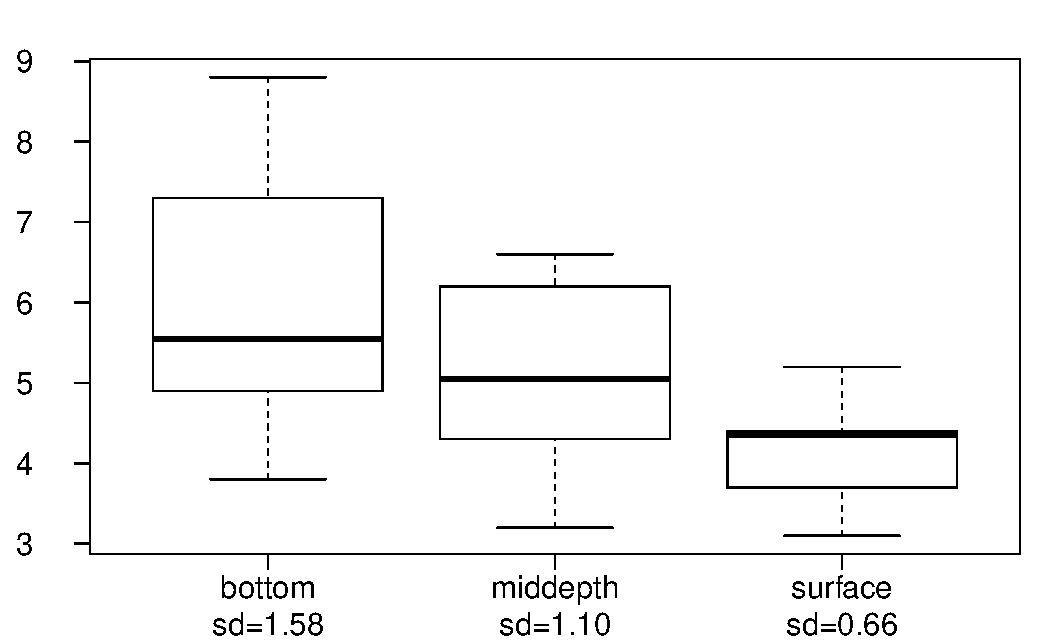
\includegraphics[width=\textwidth]{7-5_anova/figures/aldrin/homo}
}
{
\begin{enumerate}[(a)]
\item bottom \& surface
\item bottom \& mid-depth
\item mid-depth \& surface
\item bottom \& mid-depth; mid-depth \& surface
\item bottom \& mid-depth; bottom \& surface; mid-depth \& surface
\end{enumerate}
}

\end{frame}

%%%%%%%%%%%%%%%%%%%%%%%%%%%%%%%%%%

\begin{frame}
\frametitle{Which means differ? (cont.)}

If the ANOVA assumption of equal variability across groups is satisfied, we can use the data from all groups to estimate variability:
 
\begin{itemize}

\item Estimate any within-group standard deviation with $\sqrt{MSE}$, which is $s_{pooled}$

\item Use the error degrees of freedom, $n - k$, for $t$-distributions

\end{itemize}

\formula{Difference in two means: after ANOVA}{
\[ SE = \sqrt{  \frac{\sigma_1^2}{n_1} + \frac{\sigma_2^2}{n_2} } \approx \sqrt{ \frac{MSE}{n_1} + \frac{MSE}{n_2} } \]
}

\end{frame}

%%%%%%%%%%%%%%%%%%%%%%%%%%%%%%%%%%

\begin{frame}
\frametitle{}

\dq{Is there a difference between the  average aldrin concentration at the bottom and at mid depth?}

\twocol{0.4}{0.7}{
{\scriptsize
\begin{center}
\begin{tabular}{l | c c c}
		& n	& mean	& sd		\\
\hline
bottom	& 10	& \orange{6.04}	& 1.58 \\
middepth& 10	& \orange{5.05}	& 1.10 \\
surface	& 10	& 4.2 	& 0.66 \\
\hline
overall	& 30	& 5.1		& 1.37
\end{tabular}
\end{center}
}
}
{
{\scriptsize
\begin{center}
\begin{tabular}{l rrrrr}
\hline
 			& Df 	& Sum Sq	& Mean Sq 	& F value 	& Pr($>$F) \\ 
\hline
depth 		& 2 	& 16.96 	& 8.48 		& 6.13 	& 0.0063 \\ 
Residuals 	& \orange{27} 	& 37.33 	& \orange{1.38} 		&  		&  \\ 
\hline
Total			& 29	& 54.29 \\
\end{tabular}
\end{center}
}
}

\begin{eqnarray*}
T_{df_E} &=& \frac{(\bar{x}_{bottom} - \bar{x}_{middepth})}{\sqrt{ \frac{MSE}{n_{bottom}} + \frac{MSE}{n_{middepth}} }} \\ 
\pause
T_{27} &=& \frac{( 6.04 - 5.05 )}{\sqrt{ \frac{1.38}{10} + \frac{1.38}{10} }} = \frac{0.99}{0.53}  =1.87 \\
\pause
0.05 &<& p-value < 0.10 \qquad \text{{\footnotesize (two-sided)}} \\
\pause
\alpha^\star &=& 0.05 / 3 = 0.0167
\end{eqnarray*}

\pause
{\small Fail to reject $H_0$, data do not provide convincing evidence of a difference between average aldrin concentrations at bottom and mid depth.}

\end{frame}

%%%%%%%%%%%%%%%%%%%%%%%%%%%%%%%%%%

\begin{frame}
\frametitle{}

\app{Pairwise comparisons}{Is there a difference between the  average aldrin concentration at the bottom and at surface?}

\pause

\soln{
\begin{eqnarray*}
T_{df_E} &=& \frac{(\bar{x}_{bottom} - \bar{x}_{surface})}{\sqrt{ \frac{MSE}{n_{bottom}} + \frac{MSE}{n_{surface}} }} \\ 
\pause
T_{27} &=& \frac{( 6.04 - 4.02 )}{\sqrt{ \frac{1.38}{10} + \frac{1.38}{10} }} = \frac{2.02}{0.53}  =3.81 \\
\pause
p-value &<& 0.01 \qquad \text{{\footnotesize (two-sided)}} \\
\pause
\alpha^\star &=& 0.05 / 3 = 0.0167
\end{eqnarray*}
\pause
{\small Reject $H_0$, the data provide convincing evidence of a difference between the average aldrin concentrations at bottom and surface.}
}

\end{frame}

%%%%%%%%%%%%%%%%%%%%%%%%%%%%%%%%%%